\documentclass[portuguese,notheorems]{beamer}
\usetheme{Darmstadt}
\usepackage[utf8]{inputenc}
\usepackage[T1]{fontenc}
\usepackage{lmodern}
\usepackage[style=alphabetic]{biblatex}
\addbibresource{ref.bib}
\usepackage[portuguese]{babel}
\usepackage{amsmath}
\usepackage{amsfonts}
\usepackage{hyphsubst}
\usepackage{amssymb}
\usepackage{physics}
\usepackage{mathtools, esvect}
\usepackage{blindtext}
\usepackage{caption}
\usepackage{geometry}
\usepackage{mathtools}
\usepackage{bm}
\usepackage{subcaption}
\usepackage[font={it}]{caption}
\usepackage{tikz}
\usepackage{multirow}
\usepackage{booktabs}
\usetikzlibrary{shapes.geometric, arrows, positioning, angles, quotes}
\usetikzlibrary{decorations.pathmorphing}\usepackage{hyphenat}
\usepackage{multicol}
\usetikzlibrary{angles, quotes}
\renewcommand\familydefault{\sfdefault}
\mathtoolsset{showonlyrefs}

\usefonttheme[onlymath]{serif}
\usepackage{xcolor}
\usepackage{color}
% The following special color definitions are used in the IST Thesis
\definecolor{forestgreen}{RGB}{34,139,34}
\definecolor{orangered}{RGB}{239,134,64}
\definecolor{lightred}{rgb}{1,0.4,0.5}
\definecolor{orange}{rgb}{1,0.45,0.13}
\definecolor{darkblue}{rgb}{0.0,0.0,0.6}
\definecolor{lightblue}{rgb}{0.1,0.57,0.7}
\definecolor{gray}{rgb}{0.4,0.4,0.4}
\definecolor{lightgray}{rgb}{0.95, 0.95, 0.95}
\definecolor{darkgray}{rgb}{0.4, 0.4, 0.4}
\definecolor{editorGray}{rgb}{0.95, 0.95, 0.95}
\definecolor{editorOcher}{rgb}{1, 0.5, 0} % #FF7F00 -> rgb(239, 169, 0)
\definecolor{chaptergrey}{rgb}{0.6,0.6,0.6}
\definecolor{editorGreen}{rgb}{0, 0.5, 0} % #007C00 -> rgb(0, 124, 0)
\definecolor{olive}{rgb}{0.17,0.59,0.20}
\definecolor{brown}{rgb}{0.69,0.31,0.31}
\definecolor{purple}{rgb}{0.38,0.18,0.81}

\usepackage{hyperref}
% pre-configuration of hyperref
\hypersetup{ colorlinks=true,
             citecolor=cyan,
             linkcolor=darkgray,
             urlcolor=teal,
             breaklinks=true,
             bookmarksnumbered=true,
             bookmarksopen=true,
}



\captionsetup{font=scriptsize,labelfont=scriptsize}

\setbeamertemplate{theorems}[]
\setbeamercovered{transparent}

\newtheorem{theorem}{Teorema}
\newtheorem{corollary}[theorem]{Corolário}
\newtheorem{proposition}[theorem]{Proposição}
\newtheorem{lemma}[theorem]{Lema}
\newtheorem{definition}[theorem]{Definição}
\newtheorem{conjecture}[theorem]{Conjetura}

\DeclareMathOperator{\Span}{span}
\DeclareMathOperator{\dom}{Dom}
\DeclareMathOperator\supp{supp}
\DeclareMathOperator\Div{div}
\DeclareMathOperator{\atantwo}{atan \mspace{2mu} 2}

\usepackage{appendixnumberbeamer}
\addtobeamertemplate{navigation symbols}{}{%
    \usebeamerfont{footline}%
    \usebeamercolor[fg]{footline}%
    \hspace{1em}%
    \insertframenumber/\inserttotalframenumber
}

\setbeamercolor{footline}{fg=blue}
\setbeamerfont{footline}{series=\bfseries}
%\makeatletter
%\let\beamer@writeslidentry@miniframeson=\beamer@writeslidentry%
%\def\beamer@writeslidentry@miniframesoff{%
%  \expandafter\beamer@ifempty\expandafter{\beamer@framestartpage}{}% does not happen normally
%  {%else
%    % removed \addtocontents commands
%    \clearpage\beamer@notesactions%
%  }
%}
%\newcommand*{\miniframeson}{\let\beamer@writeslidentry=\beamer@writeslidentry@miniframeson}
%\newcommand*{\miniframesoff}{\let\beamer@writeslidentry=\beamer@writeslidentry@miniframesoff}
%\makeatother

%\renewcommand\bibsection{\section[]{\refname}}

\title{A numerical study of the Dirac Spectrum and Transmission Problems employing the
Method of Fundamental Solutions}
\author{Francisco Bento \\ \scriptsize{\vspace{0.2cm} Orientado por: \\ \vspace{0.1cm} Juha Hans Videman \\ Pedro Ricardo Simão Antunes}}
\institute{Instituto Superior Técnico - Lisboa, Portugal}
\date{11 de Outubro de 2023}

\begin{document}

\frame{\titlepage}

\section{Introdução}

\begin{frame}\frametitle{Visão geral do trabalho}
    %Nesta apresentação, seguimos a seguinte ordem:
    \begin{enumerate}
        \pause\item O Método das Soluções Fundamentais:
            \begin{itemize}
                \item Construção;
                \item Enriquecimento de base;
            \end{itemize}
        \pause\item O operador de Dirac e um problema de decomposição:
            \begin{itemize}
                \item Propriedades;
                \item Resultados relevantes;
            \end{itemize}
        \pause\item Simulações Numéricas;
        \pause\item Discussão e Conclusão.
    \end{enumerate}
\end{frame}

\section{O MSF}

\begin{frame}
    \centering
    \LARGE
    O Método das Soluções Fundamentais
\end{frame}

\begin{frame}\frametitle{O Método das Soluções Fundamentais}
    Considere-se o Problema de Valores de Fronteira (BVP em inglês)
    \[
        \begin{cases}
            \mathcal{L}u(x) = 0, & x \in \Omega\\
            \mathcal{B}u(x) = 0, & x \in \Gamma,
        \end{cases}
    \]
    onde $\Omega$ é um domínio limitado, $\mathcal{L}$ é um operador diferencial linear elíptico, \(\Gamma = \partial\Omega\) e \(\mathcal{B}\) é um operador linear sobre \(\Gamma\).
\end{frame}

\begin{frame}\frametitle{O Método das Soluções Fundamentais}
    Seja \(\hat{\Omega}\) tal que \(\overline{\Omega} \subset \hat{\Omega}\) com \(\hat{\Gamma} = \partial\hat{\Omega}\), e \(\mathcal{Y} = \{y_j \in \hat{\Gamma}: j=1,\dots,N\}\) um conjunto de \textit{pontos fonte} sobre a \textit{fronteira artificial} \(\hat{\Gamma}\).
    \pause

    No contexto do Método das Soluções Fundamentais (MSF em português, MFS em inglês), consideramos a aproximação
    \begin{equation*}
        \Tilde{u}(x) = \sum_{j=1}^{N}\alpha_j \Phi(x-y_j),
    \end{equation*}
onde os coeficientes \(\alpha_j\) podem ser determinados através do operador de fronteira
        \[
            \mathcal{B}\Tilde{u}(x) = \sum_{j=1}^{N}\alpha_j \mathcal{B}\Phi(x-y_j) = 0.
        \]
\end{frame}

\begin{frame}\frametitle{O Método das Soluções Fundamentais}
    \begin{figure}
        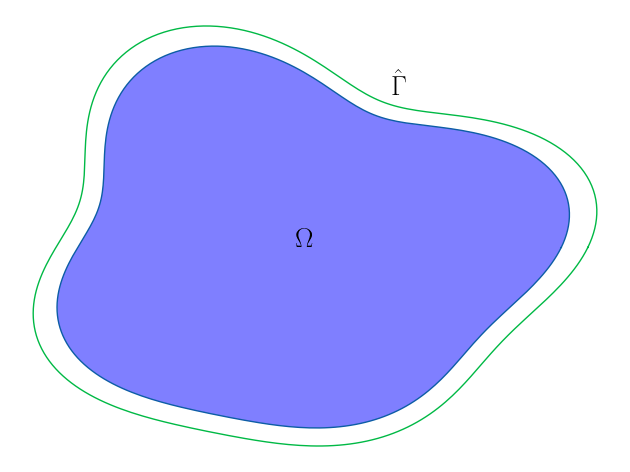
\includegraphics[scale=0.5]{configuration_art_boundary.png}
        \caption{Um domínio conexo $\Omega$ com fronteira artificial \(\hat{\Gamma}\).}
    \end{figure}
\end{frame}


\begin{frame}\frametitle{Um método de enriquecimento para a equação de Laplace}
    Para descrever o comportamento das soluções perto de um canto podemos usar \textit{soluções particulares}, soluções da equação de Laplace em coordenadas polares
    \begin{equation}
        \left(\partial_r^2 + \frac{1}{r} \partial_r +\frac{1}{r^2}\partial_\theta^2\right)u(r,\theta) = 0, \quad r>0, \; 0 \leq \theta \leq \Theta.
    \end{equation}

    \begin{figure}[H]
    \centering
    \begin{tikzpicture}[thick,scale=0.6, every node/.style={scale=0.8}]
        % Coordinates of the triangle vertices
        \coordinate[label=left:O] (O) at (0,0);
        \coordinate[label=right:A] (A) at (3,0);
        \coordinate[label=above:B] (B) at (1.5,2.5);

        % Drawing the triangle
        \draw (O) -- (A);
        \draw (O) -- (B);
        % Labeling the angle
        \draw (0.6,0) arc (0:60:0.6);
        \node at (0.8,0.3) {$\Theta$};
        \draw [decorate, decoration={snake, amplitude=0.3mm, segment length=4.5mm}] (A) to[out=45, in=0] (B);
    \end{tikzpicture}
        \caption{Um domínio com um canto com ângulo interior \(\Theta\).}
    \end{figure}
\end{frame}

\begin{frame}\frametitle{Um método de enriquecimento para a equação de Laplace}
    Por separação de variáveis, \(u(r, \theta) = R(r) T(\theta)\), temos as duas famílias de soluções particulares
\[
    u(r,\theta) = \left(c_1 r^\alpha + c_2 r^{-\alpha}\right) \times \left(c_3 \cos(\alpha \theta) + c_4 \sin(\alpha \theta)\right), \; \alpha >0
\]
ou
\[
    u(r,\theta) = \left(c_1 \log (r) + c_2 \right) \times \left(c_3 \theta + c_4 \right),
\]
    onde \(c_1, c_2, c_3, c_4 \in \mathbb{R}\) e \(\alpha\) depende das condições de fronteira e de \(\Theta\).
\end{frame}

\begin{frame}\frametitle{Um método de enriquecimento para a equação de Laplace}
    Expandindo a aproximação com as soluções particulares,
    \begin{equation}
        \tilde{u}(x) = \sum_{j=1}^{N}\alpha_j \Phi(x-y_j) + \sum_{s=1}^{P} \beta_s \phi_s(r(x),\theta(x)), \; x \in \overline{\Omega},
    \end{equation}
    onde \(\phi_s\) é a forma geral de cada solução particular, centrada no canto.
\end{frame}

\section{O operador de Dirac}
\begin{frame}
    \centering
    \LARGE
    O operador de Dirac
\end{frame}

\begin{frame}\frametitle{O operador de Dirac}
    Seja \(\Omega \subset \mathbb{R}^2\) um domínio Lipschitz com fronteira \(\Gamma\), e \(m \geq 0\). O operador de Dirac é dado pelo Hamiltoniano
    \begin{equation}
        \hat{H}=\begin{bmatrix}
        m & -i(\partial_1 - i \partial_2)\\
        -i(\partial_1 + i \partial_2) & -m
    \end{bmatrix}
\end{equation}
cujo domínio é dado por
\[
\dom(\hat{H}) = \{\mathbf{u} \in H^1(\Omega, \mathbb{C}^2): u_2 = i(n_1+i n_2)u_1 \text{ em } \Gamma\}
\]
onde $\mathbf{n}=(n_1,n_2)$ é a normal unitária exterior em cada ponto $x \in \Gamma$.

\pause
    Estudamos a solução \(\mathbf{u} = \begin{bmatrix} u_1(x) \\ u_2(x)\end{bmatrix}\) da equação (de Dirac)
    \[
        \hat{H}\mathbf{u} = \lambda \mathbf{u}
    \]
    em \(\dom(\hat{H})\).
\end{frame}

\begin{frame}\frametitle{O operador de Dirac}
    Após algumas manipulações, a equação de Dirac pode ser transformada na equação de Helmholtz com condições de fronteira de Cauchy-Riemann oblíquas
        \begin{equation}
        \begin{cases}
            -\Delta u_1 = (\lambda^2 - m^2)u_1, & \text{ em } \Omega\\
             i (\partial_1 + i\partial_2)u_1 + (\lambda + m)i(n_1 + i n_2)u_1 = 0, & \text{ em } \Gamma,
        \end{cases}
    \end{equation}
    e
        \[
    u_2 = \frac{-i (\partial_1 + i\partial_2)u_1}{\lambda + m}.
    \]

\end{frame}

\begin{frame}\frametitle{O operador de Dirac (conjeturas a estudar)}
    \begin{conjecture}[Uma conjetura do tipo Faber-Krahn]
        Seja \(\Omega \subset \mathbb{R}^2\) um domínio Lipschitz. Então,
    \[
    \lambda_1(\Omega) \geq \lambda_1(\Omega^\ast)
    \]
    onde \(\Omega^\ast\) é o disco com a mesma área ou perímetro de \(\Omega\).
\end{conjecture}
\pause
\begin{conjecture}[Uma conjetura do tipo Ashbaugh-Benguria]
    Seja \(\Omega \subset \mathbb{R}^2\) um domínio Lipschitz. Então, a solução para o problema de maximização
    \[
    \max \Big\{\frac{\lambda_2(\Omega)}{\lambda_1(\Omega)}: \Omega \subset \mathbb{R}^2\Big\}
    \]
    é a bola em \(\mathbb{R}^2\).
\end{conjecture}

\end{frame}

\begin{frame}\frametitle{O operador de Dirac (conjeturas a estudar)}
    \begin{conjecture}[Otimização de forma em retângulos]
        Seja \(\lambda_1(a, b) = \lambda_1(\Omega_{a, b})\) o primeiro valor próprio do operador de Dirac com condições de massa infinita num retângulo de lados \(a\) e \(b\). Então,
        \begin{enumerate}
            \item \label{david_conjectures_1} \textit{Restrição de área (unitária): } \[\lambda_1(a, \frac{1}{a}) \geq \lambda_1(1, 1), \; \forall a>0; \]
            \item  \label{david_conjectures_2} \textit{Restrição de perímetro (igual a 4): } \[\lambda_1(a, 2-a) \geq \lambda_1(1, 1), \; \forall a\in (0, 2).\]
        \end{enumerate}
    \end{conjecture}
\end{frame}


\begin{frame}\frametitle{O operador de Dirac (conjeturas a estudar)}
    \begin{conjecture}[Otimização de forma em triângulos]
        Considere-se o triângulo \(\Omega_{a, b}\) definindo pelos pontos \(O=(0, 0), A=(a, 0)\) e \(B=(0, b)\) com \(a, b>0\) e seja \(\lambda_1(a, b) = \lambda_1(\Omega_{a, b})\). Então,
        \begin{enumerate}
        \item \textit{Restrição de área } \[\lambda_1(a, b) \geq \lambda_1(k, k),\; \forall a, b>0\] para qualquer \(k\) positivo tal que \(ab=k^2\);
        \item \textit{Restrição de perímetro } \[\lambda_1(a, b) \geq \lambda_1(k, k),\; \forall a \in (0, (2+\sqrt{2})k)\] e \(\forall b > 0\) tal que \(a+b+\sqrt{a^2+b^2}=(2+\sqrt{2})k\), para qualquer \(k\) positivo.
        \end{enumerate}
    \end{conjecture}
\end{frame}

\begin{frame}\frametitle{O operador de Dirac (conjeturas a estudar)}
    \begin{conjecture}\label{polya_szego_conjecture_dirac}
        Seja \(\Omega \subset \mathbb{R}^2\) um aberto Lipschitz, \(n \geq 5\) e considere-se a classe dos polígonos de \(n\) lados. Então, o polígono regular de \(n\) lados tem o menor primeiro valor próprio entre todos os polígonos de \(n\) lados com área fixa.
    \end{conjecture}
\end{frame}

\section{Um problema de decomposição}

\begin{frame}
    \centering
    \LARGE
    Um problema de decomposição com condições de transmissibilidade
\end{frame}

\begin{frame}\frametitle{Problema de decomposição com condições de transmissibilidade}
    Seja \(\overline{\Omega} = \overline{\Omega}_1 \cup \overline{\Omega}_2\), \(\gamma = \partial\Omega_1 \cap \partial \Omega_2\), \(\Gamma_i = \partial\Omega_i \setminus \gamma\) e \(\mathbf{n} = \mathbf{n}_1 = -\mathbf{n}_2\) a normal unitária de \(\Omega_i\) quando restringido a \(\gamma\), para \(i=1,2\). Para os coeficientes materiais \(k_1 \geq k_2 > 0\) e \(f_i \in L^2(\Omega_i)\), consideramos

    \begin{columns}[T] % align columns
        \begin{column}{.48\textwidth}
        \centering
            \begin{figure}
            \begin{tikzpicture}[scale=0.7]
                % Draw left square and label
                \draw (0,0) rectangle (3,3);
                \node at (1.5,1.5) {\(\Omega_1\)};
                \node[below] at (1.5,0) {\(\Gamma_1\)};

                % Draw dashed interface line and label
                \draw[dashed] (3,0) -- (3,3);
                \node at (3.2,1.5) {\(\gamma\)};

                % Draw right square and label
                \draw (3,0) rectangle (6,3);
                \node at (4.5,1.5) {\(\Omega_2\)};
                \node[below] at (4.5,0) {\(\Gamma_2\)};
            \end{tikzpicture}
            \caption{Possível configuração do problema de transmissão}
            \end{figure}
        \end{column}%
        \hfill%
        \begin{column}{.48\textwidth}
        \begin{align}\label{decomp_prob}
            \begin{cases}
                - \div \left(k_i \nabla u_i\right) = f_i, & \text{em }\Omega_i\\
                u_1 - u_2 = 0, & \text{em }\gamma\\
                k_1 \frac{\partial u_1}{\partial \mathbf{n_1}} + k_2 \frac{\partial u_2}{\partial  \mathbf{n_2}} = 0, & \text{em }\gamma\\
                u_i = 0, & \text{em }\Gamma_i,
            \end{cases}
        \end{align}
        \end{column}%
        \end{columns}
\end{frame}


\section{Simulações Numéricas}

\begin{frame}
    \centering
    \LARGE
    Simulações Numéricas
\end{frame}

\begin{frame}\frametitle{Simulações Numéricas (operador de Dirac)}
    \centering Resultados para retângulos com área fixa:
\begin{figure}
    \centering
    \begin{minipage}{.52\textwidth}
      \centering
      \includegraphics[width=\linewidth]{/home/francisco/Universidade/Tese/Report/Report/Images/Dirac/quad/eigenvalues_rectangle_width_m_1.png}
      \captionsetup{width=0.9\linewidth} % Adjust the width of the caption
      \captionof{figure}{Comportamento dos primeiros cinco valores próprios para retângulos de área unitária, comprimento \(a\) e \(m=1\).}
    \end{minipage}%
    %\hspace{0.5cm} % Add some horizontal space between the figures
    \begin{minipage}{.52\textwidth}
      \centering
      \includegraphics[width=1\linewidth]{/home/francisco/Universidade/Tese/Report/Report/Images/Dirac/quad/eigenvalues_rectangle_width_m_5.png}
      \captionsetup{width=0.9\linewidth} % Adjust the width of the caption
      \captionof{figure}{Comportamento dos primeiros cinco valores próprios para retângulos de área unitária, comprimento \(a\) e \(m=5\).}
    \end{minipage}
\end{figure}
\end{frame}

\begin{frame}\frametitle{Simulações Numéricas (operador de Dirac)}
    \centering Resultados para retângulos com perímetro fixo:
\begin{figure}
    \centering
    \begin{minipage}{.52\textwidth}
      \centering
      \includegraphics[width=\linewidth]{/home/francisco/Universidade/Tese/Report/Report/Images/Dirac/quad/eigenvalues_rectangle_perimeter_width_m_1.png}
      \captionsetup{width=0.9\linewidth} % Adjust the width of the caption
      \captionof{figure}{Comportamento dos primeiros cinco valores próprios para retângulos de perímetro 4, comprimento \(a\) e \(m=1\).}
    \end{minipage}%
    %\hspace{0.5cm} % Add some horizontal space between the figures
    \begin{minipage}{.52\textwidth}
      \centering
      \includegraphics[width=1\linewidth]{/home/francisco/Universidade/Tese/Report/Report/Images/Dirac/quad/eigenvalues_rectangle_perimeter_width_m_5.png}
      \captionsetup{width=0.9\linewidth} % Adjust the width of the caption
      \captionof{figure}{Comportamento dos primeiros cinco valores próprios para retângulos de perímetro 4, comprimento \(a\) e \(m=5\).}
    \end{minipage}
\end{figure}
\end{frame}


\begin{frame}\frametitle{Simulações Numéricas (operador de Dirac)}
    \begin{figure}
    \centering Resultados para quadriláteros com área fixa e $m=1$:
        \centering
        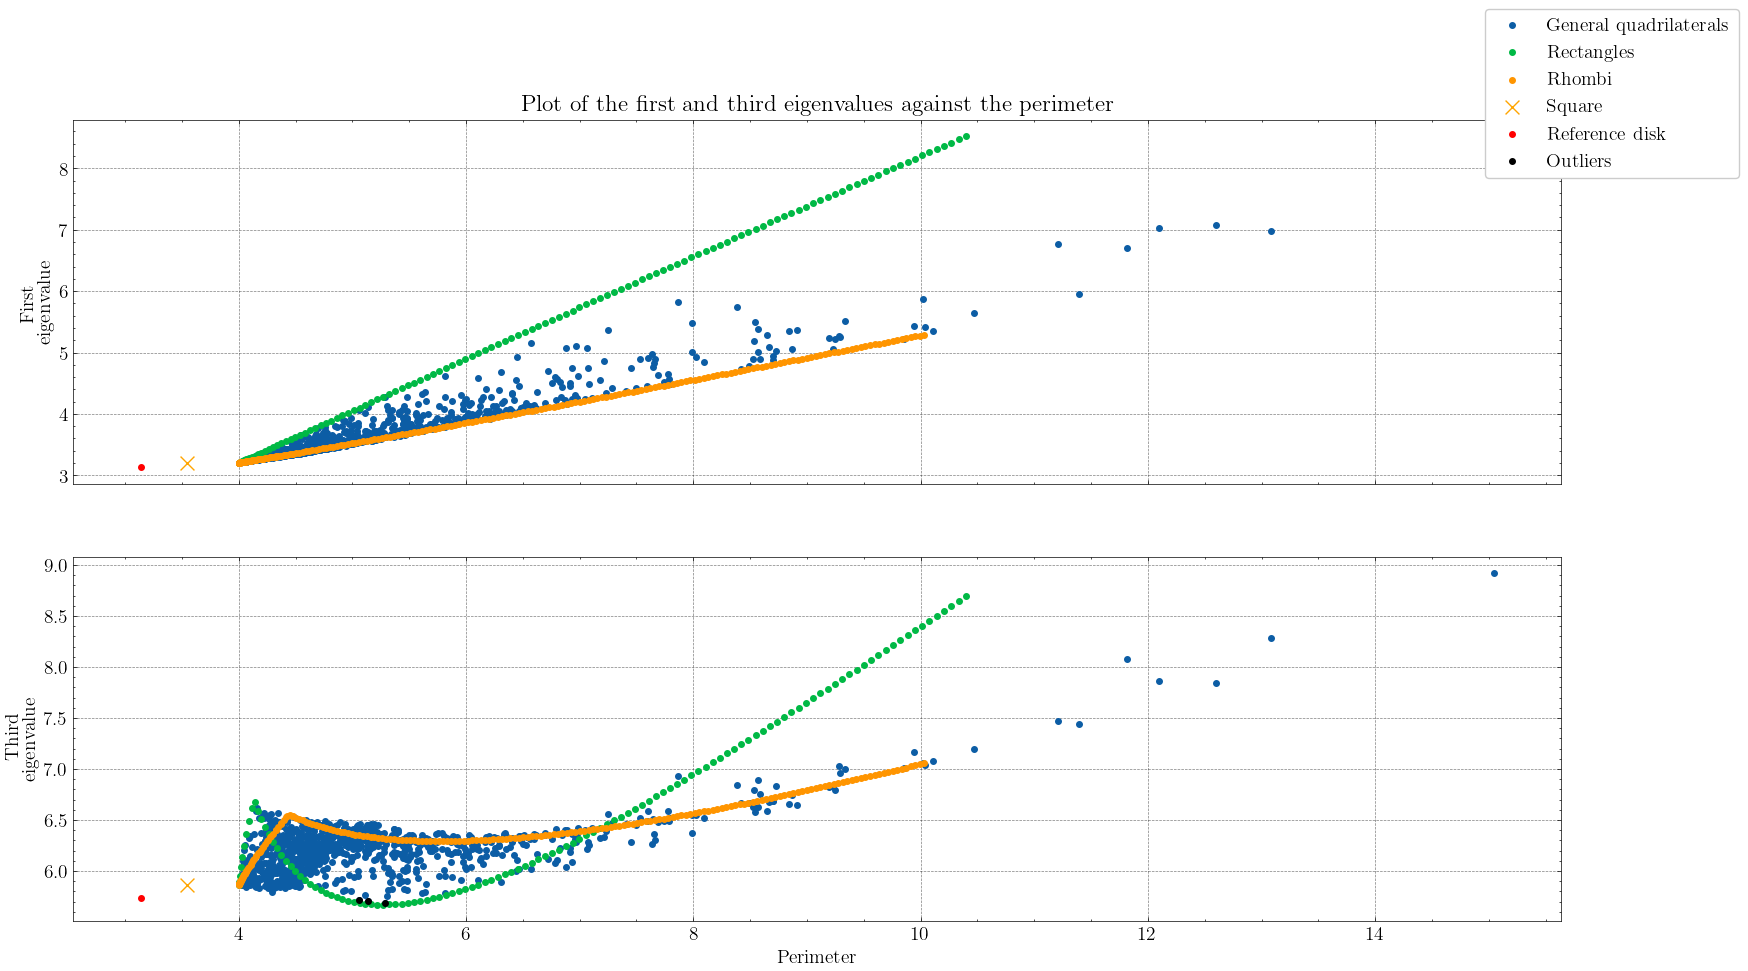
\includegraphics[width=0.9\textwidth]{/home/francisco/Universidade/Tese/Report/Beamer/quad_first_and_third.png}
        \caption{Resultados para os três primeiros valores próprios de quadriláteros aleatórios em função do perímetro para $m=1$. A preto, encontram-se representados os domínios cujos terceiro valor próprio é menos que o terceiro valor próprio do disco.}
    \end{figure}
\end{frame}

\begin{frame}\frametitle{Simulações Numéricas (operador de Dirac)}
    \centering Rácio entre $\lambda_2$ e $\lambda_1$ para $m=1$.
\begin{figure}
    \centering
      \includegraphics[width=0.6\textwidth]{/home/francisco/Universidade/Tese/Report/Report/Images/Dirac/quad/benguria_quad.png}
      \captionsetup{width=0.9\linewidth} % Adjust the width of the caption
      \captionof{figure}{Rácio $\frac{\lambda_2}{\lambda_1}$ em função do perímetro de quadriláteros aleatórios, para $m=1$.}
\end{figure}
\end{frame}

\begin{frame}\frametitle{Simulações Numéricas (operador de Dirac)}
    De forma a abordar a conjetura para triângulos, consideramos a seguinte região de triângulos admissíveis:
    \begin{figure}
        \centering
        \includegraphics[width=0.5\linewidth]{/home/francisco/Universidade/Tese/Report/Report/Images/Dirac/model_triangle.png}
        \caption{Espaço de configuração de regiões admissíveis (representada por $R$). A linha vermelha a tracejado representa um triângulo \textit{subequilátero}; a tracejado azul, um triângulo \textit{superequilátero}.}
    \end{figure}
\end{frame}

\begin{frame}\frametitle{Simulações Numéricas (operador de Dirac)}
    Resultados para triângulos com área fixa e $m=1$:
    \begin{figure}[h]
    \centering
    \begin{minipage}{.45\textwidth}
      \centering
        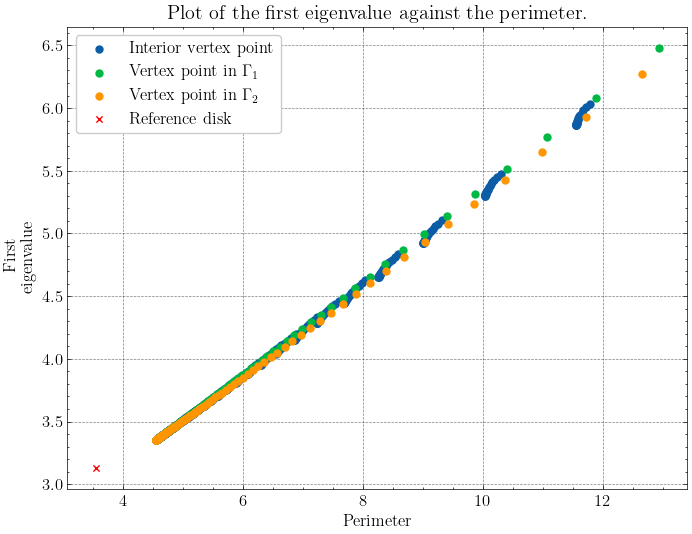
\includegraphics[width=\textwidth]{/home/francisco/Universidade/Tese/Report/Beamer/triangle_fixed_area.png}
      \captionsetup{width=0.9\linewidth} % Adjust the width of the caption
        \captionof{figure}{Resultado para o primeiro valor próprio de triângulos admissíveis em função do perímetro para $m=1$.}
    \label{dirac_smooth_first_eigenvalue}
\end{minipage}%
    %\hspace{0.5cm} % Add some horizontal space between the figures
    \begin{minipage}{.45\textwidth}
      \centering
      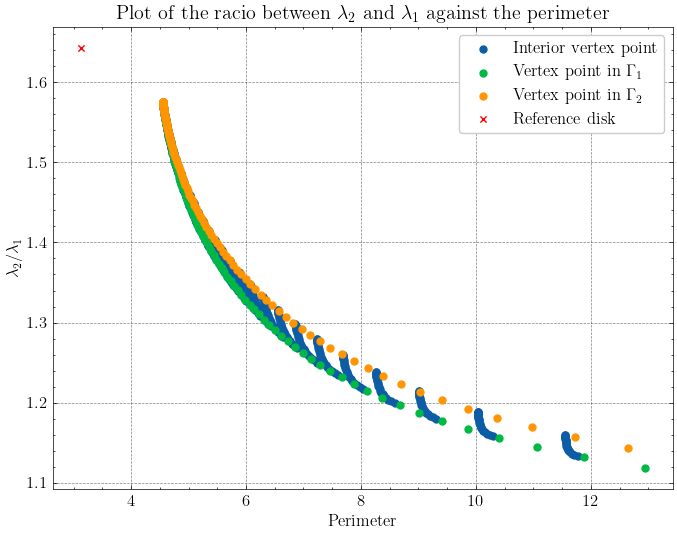
\includegraphics[width=\textwidth]{/home/francisco/Universidade/Tese/Report/Beamer/triangle_area_benguria.png}
      \captionsetup{width=0.9\linewidth} % Adjust the width of the caption
      \captionof{figure}{Ratio between the first two eigenvalues \(\frac{\lambda_2}{\lambda_1}\) for triangular domains.}
    \label{dirac_triangle_benguria}
\end{minipage}
\end{figure}
\end{frame}

%\begin{frame}\frametitle{Simulações Numéricas (operador de Dirac)}
%    Resultados para triângulos com perímetro fixo e $m=1$:
%    \begin{figure}
%    \centering
%      \centering
%        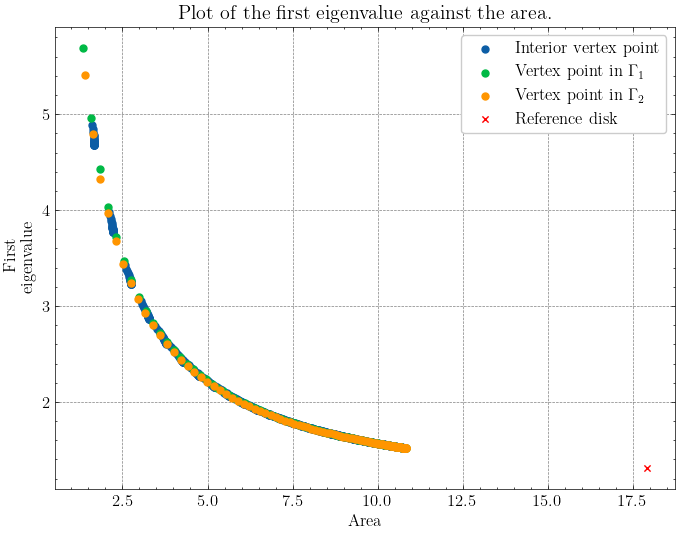
\includegraphics[width=0.5\textwidth]{/home/francisco/Universidade/Tese/Report/Beamer/triangle_fixed_perimeter.png}
%        \caption{Resultado para o primeiro valor próprio de triângulos admissíveis em função da área para $m=1$.}
%\end{figure}
%\end{frame}

\begin{frame}\frametitle{Simulações Numéricas (operador de Dirac)}
    Resultados para polígonos de $n$ lados com área fixa e $m=1$:

    \begin{figure}
        \centering
        \begin{minipage}[b]{0.3\textwidth}
            \centering
            \includegraphics[width=0.9\textwidth]{/home/francisco/Universidade/Tese/Report/Report/Images/Dirac/Polygons/pentagons.png}
            \captionsetup{width=1.5\linewidth} % Adjust the width of the caption
            \captionof{figure}{Simulações numéricas para o primeiro valor próprio de pentágonos aleatórios.}
            \label{dirac_polya_szego_evidence_pentagons}
        \end{minipage}
        \hspace*{2cm}
        \begin{minipage}[b]{0.3\textwidth}
            \centering
            \includegraphics[width=0.9\textwidth]{/home/francisco/Universidade/Tese/Report/Report/Images/Dirac/Polygons/hexagons.png}
                  \captionsetup{width=1.5\linewidth} % Adjust the width of the caption
                  \captionof{figure}{Simulações numéricas para o primeiro valor próprio de hexágonos aleatórios.}
                  \label{dirac_polya_szego_evidence_hexagons}
        \end{minipage}
    \end{figure}
    \vspace*{-0.9cm}
    \begin{figure}
        \centering
        \begin{minipage}[b]{0.3\textwidth}
            \centering
            \includegraphics[width=0.9\textwidth]{/home/francisco/Universidade/Tese/Report/Report/Images/Dirac/Polygons/heptagons.png}
                  \captionsetup{width=1.5\linewidth} % Adjust the width of the caption
                  \captionof{figure}{Simulações numéricas para o primeiro valor próprio de heptágonos aleatórios.}
            \label{dirac_polya_szego_evidence_heptagons}
        \end{minipage}
        \hspace*{2cm}
        \begin{minipage}[b]{0.3\textwidth}
            \centering
            \includegraphics[width=0.9\textwidth]{/home/francisco/Universidade/Tese/Report/Report/Images/Dirac/Polygons/octagons.png}
                  \captionsetup{width=1.5\linewidth} % Adjust the width of the caption
                  \captionof{figure}{Simulações numéricas para o primeiro valor próprio de octógonos aleatórios.}
            \label{dirac_polya_szego_evidence_octagons}
        \end{minipage}
    \end{figure}
\end{frame}


\begin{frame}\frametitle{Simulações Numéricas (operador de Dirac)}
    Por fim, procuramos a forma ótima para o terceiro valor próprio, provando não ser o disco.
    \begin{figure}
    \centering
    \begin{minipage}{.56\textwidth}
        \centering
        \includegraphics[width=0.9\linewidth]{/home/francisco/Universidade/Tese/Report/Report/Images/Dirac/smooth/nelder_mead_optimal.png}
        \captionsetup{width=0.8\linewidth} % Adjust the width of the caption
        \captionof{figure}{Domínio ótimo $\Omega^\star$ (a laranja) e o domínio original (a azul) usado para iniciar o método de Nelder-Mead.}
        \label{dirac_nelder_mead_domain}
    \end{minipage}%
    %\hspace{0.5cm} % Add some horizontal space between the figures
    \begin{minipage}{.56\textwidth}
        \centering
        \includegraphics[width=0.8\linewidth]{/home/francisco/Universidade/Tese/Report/Report/Images/Dirac/smooth/dirac_val_third.png}
        \captionsetup{width=0.8\linewidth} % Adjust the width of the caption
        \captionof{figure}{Os primeiros três valores próprios dos domínios definidos através da soma de Minkowski entre o disco e o domínio ótimo $\Omega^\star$.}
        \label{dirac_val_third}
    \end{minipage}
\end{figure}
\end{frame}

\begin{frame}\frametitle{Simulações Numéricas (problema de transmissão)}
    Transformamos o problema de transmissão numa EDP homogénea
    \begin{align}
        \begin{cases}
        - \div \left(k_i \nabla u_i^H\right)  = 0, & \text{em }\Omega_i\\
        u_1^H - u_2^H = u_2^{NH}- u_1^{NH}, & \text{em }\gamma\\
        k_1 \frac{\partial u_1^H}{\partial \mathbf{n_1}} - k_2 \frac{\partial u_2^H}{\partial  \mathbf{n_1}} = k_2 \frac{\partial u_2^{NH}}{\partial  \mathbf{n_1}}  - k_1 \frac{\partial u_1^{NH}}{\partial  \mathbf{n_1}}, & \text{em }\gamma\\
        u_i^H = - u_i^{NH}, & \text{em }\Gamma_i,
        \end{cases}
    \end{align}
    onde $k_1$ e $k_2$ são coeficientes materiais.
    \pause

    A solução final pode ser recuperada obtendo uma solução não homogénea dada por
    \[u_i = u_i^H + u_i^{NH}, \, i = 1, 2.\]
\end{frame}

\begin{frame}\frametitle{Simulações Numéricas (problema de transmissão)}
    O erro é calculado descretizando a norma de \(L^2\) na \textit{Root mean squared error} (RMSE) dada por
    \[
    \norm*{u-\tilde{u}}= \sqrt{\frac{1}{\#\mathcal{I}} \sum_{z \in \mathcal{I}} \abs{u(z)-\tilde{u}(z)}^2},
    \]
    \pause
    onde medimos os erros de consistência
    \begin{itemize}
        \item \(\norm*{\tilde{u}_i - 0}_{L^2(\Gamma_i)}\), \(i=1, 2\): erro de colocação na fronteira;
        \item \(e_\gamma^0 = \norm*{\tilde{u}_1 - \tilde{u}_2}_{L^2(\gamma)}\), \(i=1, 2\): \(L^2\) erro de \(\tilde{u}\) ao longo de \(\gamma\);
        \item \(e_\gamma^1 = \norm*{k_1 \partial_n\tilde{u}_1 - k_2 \partial_n\tilde{u}_2}_{L^2(\gamma)}\), \(i=1, 2\): \(L^2\) erro de \(\partial_n\tilde{u}\) ao longo de  \(\gamma\).
    \end{itemize}
\end{frame}

\begin{frame}\frametitle{Simulações Numéricas (problema de transmissão)}
    Resultados para retângulos:
    \begin{table}
        \centering
        \scriptsize % Reduce the font size
        \setlength{\tabcolsep}{2pt} % Reduce the column spacing
        \begin{tabular}{@{}cccccc@{}}
          \toprule
          \multirow{2}{*}{\textbf{\(k_1\) value}} & \multicolumn{2}{c}{\textbf{Boundary Error}} & \multicolumn{2}{c}{\textbf{Interface Errors}} \\
          \cmidrule(lr){2-3} \cmidrule(lr){4-5}
          & \textbf{$\partial\Omega_1$} & \textbf{$\partial\Omega_2$} & \textbf{\(e_\gamma^0\)} & \textbf{\(e_\gamma^1\)} & \\
          \midrule
          1 & $7.775\times10^{-8}$ & $7.779\times10^{-8}$ & $4.732\times10^{-9}$ & $7.589\times10^{-9}$\\
          2 & $4.398\times10^{-8}$ & $8.614\times10^{-8}$ & $2.499\times10^{-6}$ & $7.868\times10^{-8}$\\
          5 & $2.181\times10^{-8}$ & $1.036\times10^{-7}$ & $3.838\times10^{-6}$ & $1.551\times10^{-7}$\\
          \bottomrule
        \end{tabular}
        \caption{Erros de consistência na fronteira e na interface \(\gamma\).}
        \label{tab:transmission_results_rectangle}
    \end{table}
    \begin{minipage}{0.6\textwidth} % Adjust the width as needed
        \centering
        \includegraphics[width=0.7\linewidth]{/home/francisco/Universidade/Tese/Report/Report/Images/Transmission/Rectangle_contour_600_150_k1_2.png}
    \end{minipage}%
    \begin{minipage}{0.4\textwidth} % Adjust the width as needed
        \captionof{figure}{Simulações numéricas para \(k_1=2\).}
    \end{minipage}
\end{frame}

%\begin{frame}\frametitle{Simulações Numéricas (problema de transmissão)}
%    Resultados para uma L-shape com interface em \(x=0\):
%    \begin{table}
%        \centering
%        \scriptsize % Reduce the font size
%        \setlength{\tabcolsep}{2pt} % Reduce the column spacing
%        \begin{tabular}{@{}cccccc@{}}
%          \toprule
%          \multirow{2}{*}{\textbf{\(k_1\) value}} & \multicolumn{2}{c}{\textbf{Boundary Error}} & \multicolumn{2}{c}{\textbf{Interface Errors}} \\
%          \cmidrule(lr){2-3} \cmidrule(lr){4-5}
%          & \textbf{Domain 1} & \textbf{Domain 2} & \textbf{\(e_\gamma^0\)} & \textbf{\(e_\gamma^1\)} & \\
%          \midrule
%          1 & $7.853\times10^{-5}$ & $1.155\times10^{-4}$ & $2.916\times10^{-3}$ & $2.155\times10^{-5}$ \\
%          2 & $8.152\times10^{-5}$ & $1.350\times10^{-4}$ & $3.835\times10^{-3}$ & $1.149\times10^{-5}$\\
%          5 & $7.079\times10^{-5}$ & $1.378\times10^{-4}$ & $4.085\times10^{-3}$ & $5.411\times10^{-5}$\\
%          \bottomrule
%        \end{tabular}
%        \caption{Erros de consistência na fronteira e na interface \(\gamma\).}
%        \label{tab:transmission_results_L_shape_rectangles}
%    \end{table}
%    \begin{minipage}{0.6\textwidth} % Adjust the width as needed
%        \centering
%        \includegraphics[width=0.7\linewidth]{/home/francisco/Universidade/Tese/Report/Report/Images/Transmission/L_shape_2_rectangles_k1_5.png}
%    \end{minipage}%
%    \begin{minipage}{0.4\textwidth} % Adjust the width as needed
%        \captionof{figure}{Simulações numéricas para \(k_1=5\).}
%    \end{minipage}
%\end{frame}
%
%\begin{frame}\frametitle{Simulações Numéricas (problema de transmissão)}
%    Resultados para uma L-shape com interface em \(x=0\), após enriquecimento de base usando soluções particulares do tipo Dirichlet-Neumann (\(p_1\)):
%    \begin{table}
%        \centering
%        \scriptsize % Reduce the font size
%        \setlength{\tabcolsep}{2pt} % Reduce the column spacing
%        \begin{tabular}{cccccc}
%            \toprule
%            \multicolumn{1}{c}{\textbf{\(p_1\) values}} & \multicolumn{1}{c}{\textbf{\(k_1\) value}} & \multicolumn{2}{c}{\textbf{Boundary Error}} & \multicolumn{2}{c}{\textbf{Interface Errors}} \\
%            \cmidrule(lr){2-2} \cmidrule(lr){3-4} \cmidrule(lr){5-6}
%            & & \textbf{Domain 1} & \textbf{Domain 2} & \textbf{\(e_\gamma^0\)} & \textbf{\(e_\gamma^1\)} \\
%            \midrule
%
%            % Data for p = [0, 1]
%            0, 1 & 1 & $2.965\times10^{-5}$ & $7.907\times10^{-5}$ & $2.94\times10^{-3}$ & $2.624\times10^{-5}$ \\
%            & 2 & $2.203\times10^{-5}$ & $6.657\times10^{-5}$ & $1.86\times10^{-3}$ & $2.068\times10^{-5}$ \\
%            & 5 & $2.203\times10^{-5}$ & $6.657\times10^{-5}$ & $1.86\times10^{-3}$ & $2.068\times10^{-5}$ \\
%            \midrule
%
%            % Data for p = [-1, 0, 1]
%            -1, 0, 1 & 1 & $8.627\times10^{-6}$ & $4.132\times10^{-5}$ & $7.68\times10^{-4}$ & $6.876\times10^{-6}$ \\
%            & 2 & $7.333\times10^{-6}$ & $2.791\times10^{-5}$ & $6.01\times10^{-4}$ & $2.555\times10^{-5}$ \\
%            & 5 & $4.271\times10^{-6}$ & $1.118\times10^{-5}$ & $2.69\times10^{-4}$ & $4.166\times10^{-5}$ \\
%            \midrule
%
%            % Data for p = [-2, -1, 0, 1]
%            -2, -1, 0, 1 & 1 & $3.898\times10^{-6}$ & $5.975\times10^{-6}$ & $1.44\times10^{-3}$ & $2.505\times10^{-6}$ \\
%            & 2 & $2.584\times10^{-6}$ & $2.514\times10^{-6}$ & $9.69\times10^{-4}$ & $1.048\times10^{-5}$ \\
%            & 5 & $1.119\times10^{-6}$ & $6.838\times10^{-7}$ & $4.89\times10^{-4}$ & $1.106\times10^{-5}$ \\
%            \bottomrule
%        \end{tabular}
%        \caption{Erros de consistência na fronteira e na interface \(\gamma\) após enriquecimento de base com soluções particulares.}
%        \label{tab:transmission_results_L_shape_rectangles_particular}
%    \end{table}
%\end{frame}

\begin{frame}\frametitle{Simulações Numéricas (problema de transmissão)}
    Resultados para uma L-shape com interface no eixo de simetria:
    \begin{table}
        \centering
        \scriptsize % Reduce the font size
        \setlength{\tabcolsep}{2pt} % Reduce the column spacing
        \begin{tabular}{cccccc}
            \toprule
            \multirow{2}{*}{\textbf{\(k_1\) value}} & \multicolumn{2}{c}{\textbf{Boundary Error}} & \multicolumn{2}{c}{\textbf{Interface Errors}} \\
            \cmidrule(lr){2-3} \cmidrule(lr){4-5}
            & \textbf{$\partial\Omega_1$} & \textbf{$\partial\Omega_2$} & \textbf{\(e_\gamma^0\)} & \textbf{\(e_\gamma^1\)} \\
            \midrule
            1 & $1.812\times10^{-4}$ & $2.060\times10^{-4}$ & $7.305\times10^{-3}$ & $8.018\times10^{-5}$ \\
            2 & $1.398\times10^{-4}$ & $9.729\times10^{-5}$ & $5.986\times10^{-4}$ & $5.505\times10^{-5}$ \\
            5 & $7.096\times10^{-5}$ & $3.030\times10^{-5}$ & $1.528\times10^{-3}$ & $4.348\times10^{-5}$ \\
            \bottomrule
        \end{tabular}
        \caption{Erros de consistência na fronteira e na interface \(\gamma\).}
        \label{tab:transmission_results_L_shape_axis}
    \end{table}
    \begin{minipage}{0.6\textwidth} % Adjust the width as needed
        \centering
        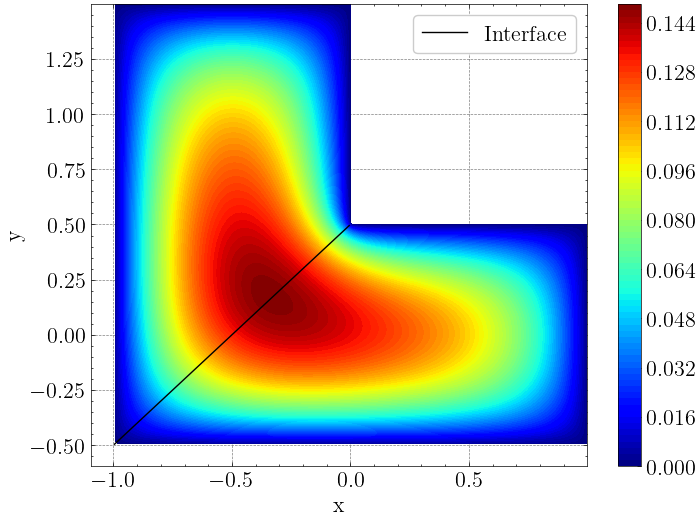
\includegraphics[width=0.75\linewidth]{/home/francisco/Universidade/Tese/Report/Beamer/l_shape_axis.png}
    \end{minipage}%
    \begin{minipage}{0.4\textwidth} % Adjust the width as needed
        \captionof{figure}{Simulações numéricas para \(k_1=1\).}
    \end{minipage}
\end{frame}

\begin{frame}\frametitle{Simulações Numéricas (problema de transmissão)}
    Resultados para uma L-shape com interface no eixo de simetria, após enriquecimento de base usando soluções particulares do tipo Dirichlet-Neumann (\(p_1\)) e Neumann-Dirichlet (\(p_2 = (0, 1)\)):
    \begin{table}
        \centering
        \scriptsize % Reduce the font size
        \setlength{\tabcolsep}{2pt} % Reduce the column spacing
        \begin{tabular}{cccccc}
            \toprule
            \multicolumn{1}{c}{\textbf{\(p_1\) values}} & \multicolumn{1}{c}{\textbf{\(k_1\) value}} & \multicolumn{2}{c}{\textbf{Boundary Error}} & \multicolumn{2}{c}{\textbf{Interface Errors}} \\
            \cmidrule(lr){2-2} \cmidrule(lr){3-4} \cmidrule(lr){5-6}
            & & \textbf{$\partial\Omega_1$} & \textbf{$\partial\Omega_2$} & \textbf{\(e_\gamma^0\)} & \textbf{\(e_\gamma^1\)} \\
            \midrule

            % Data for p = [0, 1]
            0, 1 & 1 & $2.965\times10^{-5}$ & $7.907\times10^{-5}$ & $2.94\times10^{-3}$ & $2.624\times10^{-5}$ \\
            & 2 & $2.203\times10^{-5}$ & $6.657\times10^{-5}$ & $1.86\times10^{-3}$ & $2.068\times10^{-5}$ \\
            & 5 & $2.203\times10^{-5}$ & $6.657\times10^{-5}$ & $1.86\times10^{-3}$ & $2.068\times10^{-5}$ \\
            \midrule

            % Data for p = [-1, 0, 1]
            -1, 0, 1 & 1 & $8.627\times10^{-6}$ & $4.132\times10^{-5}$ & $7.68\times10^{-4}$ & $6.876\times10^{-6}$ \\
            & 2 & $7.333\times10^{-6}$ & $2.791\times10^{-5}$ & $6.01\times10^{-4}$ & $2.555\times10^{-5}$ \\
            & 5 & $4.271\times10^{-6}$ & $1.118\times10^{-5}$ & $2.69\times10^{-4}$ & $4.166\times10^{-5}$ \\
            \midrule

            % Data for p = [-2, -1, 0, 1]
            -2, -1, 0, 1 & 1 & $3.898\times10^{-6}$ & $5.975\times10^{-6}$ & $1.44\times10^{-3}$ & $2.505\times10^{-6}$ \\
            & 2 & $2.584\times10^{-6}$ & $2.514\times10^{-6}$ & $9.69\times10^{-4}$ & $1.048\times10^{-5}$ \\
            & 5 & $1.119\times10^{-6}$ & $6.838\times10^{-7}$ & $4.89\times10^{-4}$ & $1.106\times10^{-5}$ \\
            \bottomrule
        \end{tabular}
        \caption{Erros de consistência na fronteira e na interface \(\gamma\) após enriquecimento de base com soluções particulares.}
        \label{tab:transmission_results_L_shape_axis_particular}
    \end{table}
\end{frame}

\section{Conclusão}

\begin{frame}
\frametitle{Conclusões e trabalho futuro (operador de Dirac):}
            \begin{itemize}
                \pause
                \item Provámos a  inexistência de soluções dadas por separação de variáveis usando coordenadas polares centradas num canto;
                \pause
                \item Encontrámos evidência numérica que sustenta as conjeturas de Faber-Krahn e Ashbaugh-Benguria em várias classes de domínios;
                \pause
                \item Expusemos a dependência do espetro do operador de Dirac na massa $m$;
                \pause
                \item Trabalho futuro:
                    \begin{itemize}
                        \item Resultados para outras valores próprios (por exemplo, $\lambda_2(\Omega)$);
                        \item Otimização de forma em domínios desconexos.
                    \end{itemize}
    \end{itemize}
\end{frame}
\begin{frame}
\frametitle{Conclusões e trabalho futuro (Problema de decomposição com condições de transmissão):}
    \begin{itemize}
            \pause
                \item Provámos a equivalência entre as formulações fracas da equação de Poisson com fonte descontínua e o problema de decomposição, justificando a aplicação do Método das Soluções Fundamentais;
                \pause
                \item Foi utilizada, pela primeira vez, enriquecimento de base neste tipo de problemas, diminuindo os erros de consistência em duas ordens de magnitude;
                \pause
                \item Trabalho futuro:
                    \begin{itemize}
                        \item Apresentar uma estimativa \textit{a posteriori} para o Método das Soluções Fundamentais para problemas de decomposição;
                        \item Estudar melhores formas de enriquecimento.
                    \end{itemize}
            \end{itemize}
\end{frame}

\appendix

\definecolor{mybgcolor}{RGB}{0,51,102} % Change the color as needed

\setbeamertemplate{headline}{%
  \begin{beamercolorbox}[colsep=1.5pt,wd=\paperwidth]{upper separation line head}
  \end{beamercolorbox}%
  \begin{beamercolorbox}[colsep=1.5pt,wd=\paperwidth,ht=2.5ex,dp=1.125ex]{middle separation line head}
  \end{beamercolorbox}%
  \begin{beamercolorbox}[colsep=1.5pt,wd=\paperwidth,ht=1ex,dp=0.5ex,center]{lower separation line head}
  \end{beamercolorbox}%
} % Remove the navigation bar and set background color

\begin{frame}
    \centering
    \LARGE
    Obrigado por terem assistido!

    Perguntas?
\end{frame}

\begin{frame}[allowframebreaks]{Referências}

    %\bibliographystyle{alpha}
    %\bibliography{ref.bib}

    \nocite{*}
    \printbibliography

\end{frame}

\begin{frame}
    Seja \(\mathcal{L}\) um operador linear elíptico. Dizemos que uma distribuição \( \Phi \in \mathcal{D}^\star(\mathbb{R}^d)\) é a solução fundamental da equação diferencial
    \[
        \mathcal{L}u(x) = 0, \text{ em } \mathbb{R}^d
    \]
    se \(\Phi\) satisfaz
    \[
        \mathcal{L}\Phi = \delta, \text{ em } \mathbb{R}^d
    \]
    no sentido das distribuições, onde \(\delta\) é um Delta de Dirac.
\end{frame}


\begin{frame}
    Sejam \(x_1,\ldots,x_M\) pontos de colocação sobre \(\Gamma\) e \(y_1,\ldots,y_N\) pontos fonte sobre \(\hat{\Gamma}\).

    Assumindo condições de fronteira de Dirichlet \(u=g\) em \(\Gamma\), os coeficientes \(\alpha\) são determinados resolvendo o sistema
    \begin{equation}
    {\underbrace{\begin{bmatrix}
        \Phi(x_1, y_1) & \cdots & \Phi(x_1, y_N) \\
        \vdots & \ddots & \vdots \\
        \Phi(x_M, y_1) & \cdots & \Phi(x_M, y_N)
    \end{bmatrix}}_{A}}_{M\times N}
    {\underbrace{\begin{bmatrix}
        \alpha_1\\
        \vdots\\
        \alpha_N
    \end{bmatrix}}_\alpha}_{N\times 1}
    =
    {\underbrace{\begin{bmatrix}
        g_1\\
        \vdots\\
        g_M
    \end{bmatrix}}_g}_{M\times 1}
\end{equation}
    onde \(g_i = g(x_i)\).
\end{frame}

\begin{frame}
    Considere-se o espaço funcional
        \[
        \mathcal{S}(\Gamma, \hat{\Gamma}) = \Span\{\Phi(x-y)_{|x \in \Gamma} : y \in \hat{\Gamma}\}.
        \]
    Neste trabalho, apresentamos uma variação da prova do resultado de densidade do MSF\footnote{Válido para outras condições de fronteira, para as equações de Laplace e Helmholtz.}.

    \pause
    \begin{theorem}
        Seja \(\Omega \subset \mathbb{R}^2\) um conjunto aberto, limitado e fronteira \(C^2\). Então, \(\mathcal{S}(\Gamma, \hat{\Gamma}) \oplus \mathbb{R}\) é denso em \(H^\frac{1}{2}(\Gamma)\).
    \end{theorem}
\end{frame}

\begin{frame}
    Neste trabalho, o seguinte teorema é extendido para coordenadas polares, tendo implicações no enriquecimento da base do MSF.

    \begin{theorem}
        Seja \(\mathbf{u}\in H^2(\Omega)\) a solução da equação de Dirac com condições de fronteira de massa infinita. Então, \(\mathbf{u}\) não pode ser escrita através de separação de variáveis em retângulos (coordenadas cartesianas) nem em coordenadas polares (na proximidade de um canto).
    \end{theorem}
\end{frame}


\begin{frame}
    O principal resultado relativo ao problema de decomposição refere-se à equivalência entre o problema de transmissão e a equação de Poisson com uma função fonte decontínua.

    Seja
    \[
        f = \begin{cases}
    \frac{f_1}{k_1},& \text{in } \Omega_1\\
    \frac{f_2}{k_2},& \text{in } \Omega_2.
\end{cases}
    \]
    Então, a formulação fraca da equação de Poisson
    $$
        \begin{cases}
            -\Delta u = f, &\text{em } \Omega \\
            u = 0, &\text{em } \partial\Omega
        \end{cases}
    $$
    \pause
    lê-se
    $$
        \textit{encontrar } u \in H^1_0(\Omega): \int_{\Omega} \nabla u \cdot \nabla v dx = \int_\Omega f v dx, \, \forall v \in H^1_0.
    $$
\end{frame}

\begin{frame}
Para a formulação fraca do problema de decomposição, começamos por definir os seguintes espaços de Sobolev e formas bilineares:
    \begin{align*}
        &V_i = \{v_i \in H^1(\Omega_i): v_{i_{|\partial \Omega \cap \partial {\Omega_i}}}=0\}\\,
        &V_i^0 = H^1_0(\Omega_i), \\
        &\Lambda = \{\eta \in H^\frac{1}{2}(\gamma): \eta = v_{|\gamma} \text{ para algum } v \in V^0\},\\
        &a_i (u_i, v_i) = \int_{\Omega_i} \nabla u_i \cdot \nabla v_i,\\
        &(f_i, v_i) = \int_{\Omega_i} f_i v_i dx \quad (\small \textit{produto interno de } L^2(\Omega_i)).
    \end{align*}
\end{frame}

\begin{frame}
    \begin{proposition}
    A formulação fraca do problema de transmissão pode ser lida como:
    \begin{center}
        \textit{encontrar} \(u_1\in V_1, u_2 \in V_2\) \textit{tais que}
    \end{center}
    \begin{equation*}\label{weak_decomp}
                \begin{aligned}
            &\begin{cases}
                a_1(u_1, v_1) = (\frac{f_1}{k_1}, v_1), & \forall v_1 \in V_1^0\\
                a_2(u_2, v_2) = (\frac{f_2}{k_2}, v_1), & \forall v_2 \in V_2^0\\
                u_1 = u_2, & \text{ em } \gamma\\
                \begin{aligned}
                a_1(k_1 u_1, P_1 \mu) + a_2(k_2 u_2, P_2 \mu) \\[0.2cm] = (f_1, P_1 \mu)
                + (f_2, P_2 \mu),
                \end{aligned} & \forall \mu \in \Lambda
            \end{cases}
        \end{aligned}
        \end{equation*}
\end{proposition}
\end{frame}

\begin{frame}
\frametitle{Problema de decomposição com condições de transmissibilidade}
    \begin{theorem}
        As formulações fracas da equação de Poisson e do problema de decomposição com condições de transmissibilidade são equivalentes.
    \end{theorem}
\end{frame}

\begin{frame}
    Seja:
    \begin{itemize}
      \item \(N^{(i)}\) o número de pontos fonte para o domínio \(\Omega_i\), tal que \(N=N^{(1)}+N^{(2)}\);
        \item  \(M^{(i)}\) o número de pontos de colocação na fronteira \(x^{(i)}_{m}\) para cada \(\Omega_i\) e \(M=M^{(1)}+M^{(2)}\);
        \item \(Q\) o número de pontos de colocação na interface \(z_q \in \gamma\).
    \end{itemize}
\end{frame}

\begin{frame}
    Resolvemos um sistema da forma \(A \alpha = b\) com
    \footnotesize\begin{equation*}
        A = \begin{bmatrix}
            \left[\Phi\left(x^{(1)}_{m}-y_j^{(1)}\right)\right]_{M^{(1)}\times N^{(1)}} & [0]_{M^{(1)}\times N^{(2)}} \\
            [0]_{M^{(2)}\times N^{(1)}} & \left[\Phi\left(x^{(2)}_{m}-y_j^{(2)}\right)\right]_{M^{(2)}\times N^{(2)}} \\
            \left[\Phi\left(z_q-y_j^{(1)}\right)\right]_{Q\times N^{(1)}} & \left[-\Phi\left(z_q-y_j^{(2)}\right)\right]_{Q\times N^{(2)}} \\
            \left[k_1\partial_n \Phi\left(z_q-y_j^{(1)}\right)\right]_{Q\times N^{(1)}} & \left[-k_2 \partial_n \Phi\left(z_q-y_j^{(2)}\right)\right]_{Q\times N^{(2)}}
        \end{bmatrix},
    \end{equation*}\normalsize
    e
    \footnotesize \begin{equation*}
        b = \begin{bmatrix}
        \left[-u_1^{NH}(x^{(1)}_{m})\right]_{M^{(1)}\times 1}\\
        \left[-u_2^{NH}(x^{(2)}_{m})\right]_{M^{(2)}\times 1}\\
        \left[u_2^{NH}(z_q)-u_1^{NH}(z_q)\right]_{Q\times 1}\\
        \left[k_2 \partial_n u_2^{NH}(z_q)- k_1 \partial_n u_1^{NH}(z_q)\right]_{Q\times 1}\\
    \end{bmatrix}.
\end{equation*}\normalsize
\end{frame}


\end{document}
